% Editable source for result.pdf, written by make_figures.py from run_github_38819494806/panel/result.json
\documentclass[tikz,border=6pt]{standalone}
\usepackage[T1]{fontenc}
\begin{document}
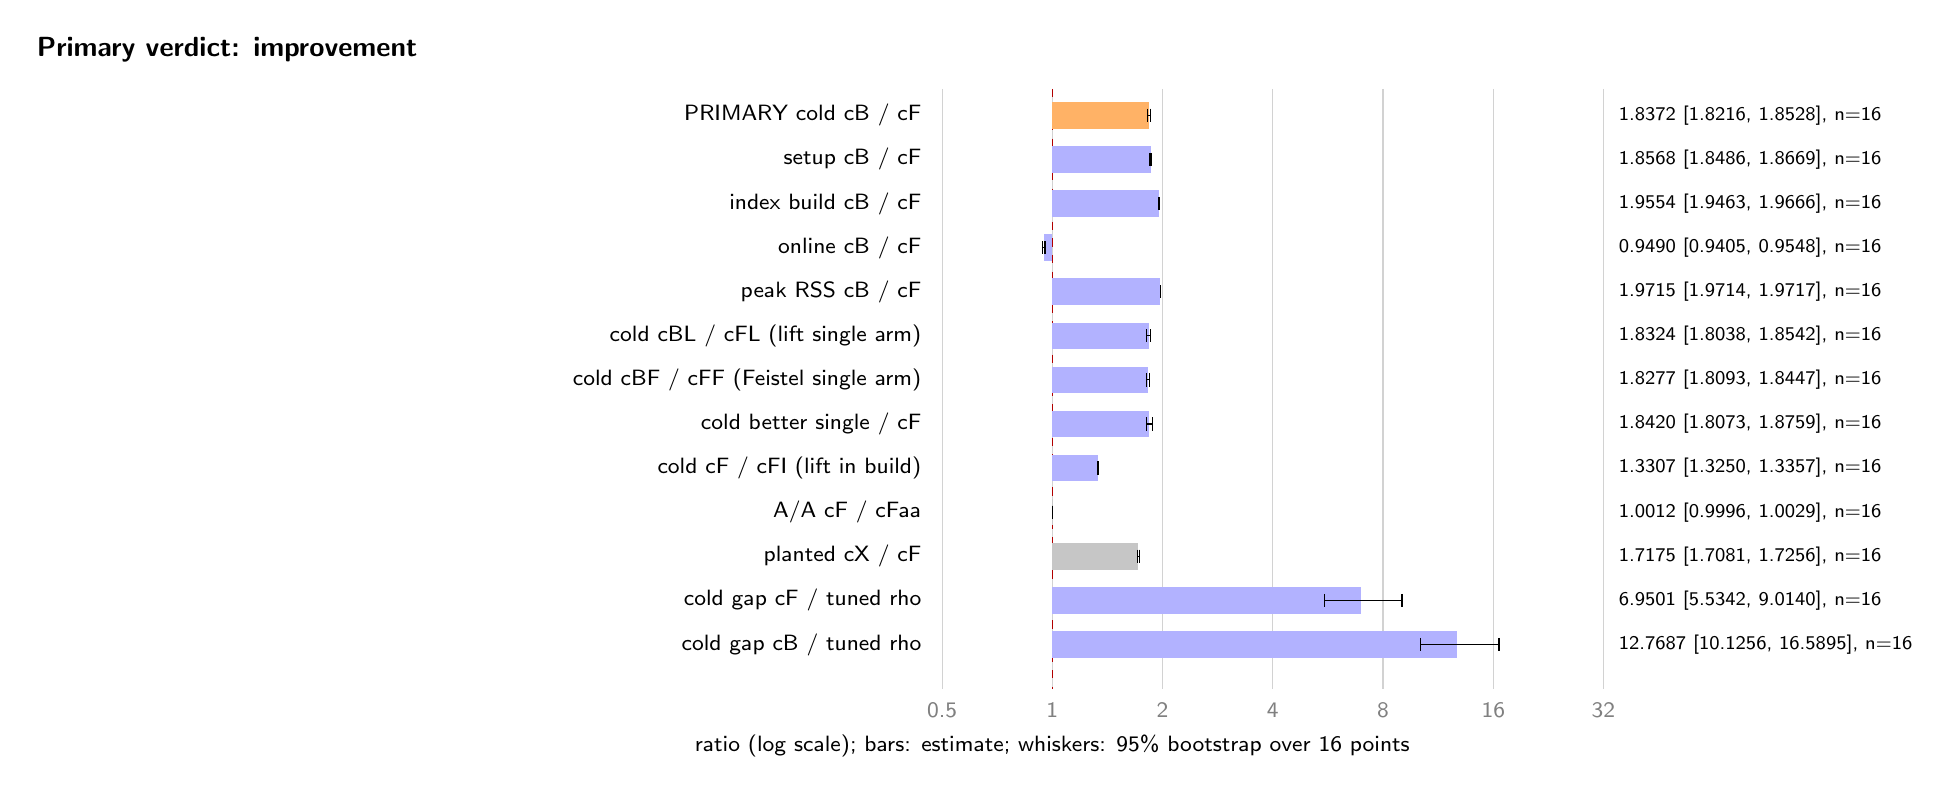
\begin{tikzpicture}[font=\sffamily\footnotesize,x=14mm,y=-5.6mm]
\draw[gray!35] (-1.0000,-0.6) -- (-1.0000,13); \node[gray] at (-1.0000,13.5) {0.5};
\draw[gray!35] (0.0000,-0.6) -- (0.0000,13); \node[gray] at (0.0000,13.5) {1};
\draw[gray!35] (1.0000,-0.6) -- (1.0000,13); \node[gray] at (1.0000,13.5) {2};
\draw[gray!35] (2.0000,-0.6) -- (2.0000,13); \node[gray] at (2.0000,13.5) {4};
\draw[gray!35] (3.0000,-0.6) -- (3.0000,13); \node[gray] at (3.0000,13.5) {8};
\draw[gray!35] (4.0000,-0.6) -- (4.0000,13); \node[gray] at (4.0000,13.5) {16};
\draw[gray!35] (5.0000,-0.6) -- (5.0000,13); \node[gray] at (5.0000,13.5) {32};
\draw[red!70!black,dashed] (0,-0.6) -- (0,13);
\node at (0,14.3) {ratio (log scale); bars: estimate; whiskers: 95\% bootstrap over 16 points};
\node[anchor=west,font=\sffamily\bfseries] at (-9.3,-1.5) {Primary verdict: improvement};
\node[anchor=east] at (-1.1000,0) {PRIMARY cold cB / cF};
\fill[orange!60] (0,-0.300000) rectangle (0.8775,0.300000);
\draw (0.8652,0) -- (0.8897,0); \draw (0.8652,-0.150000) -- (0.8652,0.150000); \draw (0.8897,-0.150000) -- (0.8897,0.150000);
\node[anchor=west,font=\sffamily\scriptsize] at (5.0500,0) {1.8372 [1.8216, 1.8528], n=16};
\node[anchor=east] at (-1.1000,1) {setup cB / cF};
\fill[blue!30] (0,0.700000) rectangle (0.8928,1.300000);
\draw (0.8864,1) -- (0.9007,1); \draw (0.8864,0.850000) -- (0.8864,1.150000); \draw (0.9007,0.850000) -- (0.9007,1.150000);
\node[anchor=west,font=\sffamily\scriptsize] at (5.0500,1) {1.8568 [1.8486, 1.8669], n=16};
\node[anchor=east] at (-1.1000,2) {index build cB / cF};
\fill[blue!30] (0,1.700000) rectangle (0.9674,2.300000);
\draw (0.9607,2) -- (0.9757,2); \draw (0.9607,1.850000) -- (0.9607,2.150000); \draw (0.9757,1.850000) -- (0.9757,2.150000);
\node[anchor=west,font=\sffamily\scriptsize] at (5.0500,2) {1.9554 [1.9463, 1.9666], n=16};
\node[anchor=east] at (-1.1000,3) {online cB / cF};
\fill[blue!30] (0,2.700000) rectangle (-0.0755,3.300000);
\draw (-0.0885,3) -- (-0.0668,3); \draw (-0.0885,2.850000) -- (-0.0885,3.150000); \draw (-0.0668,2.850000) -- (-0.0668,3.150000);
\node[anchor=west,font=\sffamily\scriptsize] at (5.0500,3) {0.9490 [0.9405, 0.9548], n=16};
\node[anchor=east] at (-1.1000,4) {peak RSS cB / cF};
\fill[blue!30] (0,3.700000) rectangle (0.9793,4.300000);
\draw (0.9792,4) -- (0.9794,4); \draw (0.9792,3.850000) -- (0.9792,4.150000); \draw (0.9794,3.850000) -- (0.9794,4.150000);
\node[anchor=west,font=\sffamily\scriptsize] at (5.0500,4) {1.9715 [1.9714, 1.9717], n=16};
\node[anchor=east] at (-1.1000,5) {cold cBL / cFL (lift single arm)};
\fill[blue!30] (0,4.700000) rectangle (0.8737,5.300000);
\draw (0.8510,5) -- (0.8908,5); \draw (0.8510,4.850000) -- (0.8510,5.150000); \draw (0.8908,4.850000) -- (0.8908,5.150000);
\node[anchor=west,font=\sffamily\scriptsize] at (5.0500,5) {1.8324 [1.8038, 1.8542], n=16};
\node[anchor=east] at (-1.1000,6) {cold cBF / cFF (Feistel single arm)};
\fill[blue!30] (0,5.700000) rectangle (0.8701,6.300000);
\draw (0.8555,6) -- (0.8834,6); \draw (0.8555,5.850000) -- (0.8555,6.150000); \draw (0.8834,5.850000) -- (0.8834,6.150000);
\node[anchor=west,font=\sffamily\scriptsize] at (5.0500,6) {1.8277 [1.8093, 1.8447], n=16};
\node[anchor=east] at (-1.1000,7) {cold better single / cF};
\fill[blue!30] (0,6.700000) rectangle (0.8812,7.300000);
\draw (0.8538,7) -- (0.9076,7); \draw (0.8538,6.850000) -- (0.8538,7.150000); \draw (0.9076,6.850000) -- (0.9076,7.150000);
\node[anchor=west,font=\sffamily\scriptsize] at (5.0500,7) {1.8420 [1.8073, 1.8759], n=16};
\node[anchor=east] at (-1.1000,8) {cold cF / cFI (lift in build)};
\fill[blue!30] (0,7.700000) rectangle (0.4122,8.300000);
\draw (0.4060,8) -- (0.4176,8); \draw (0.4060,7.850000) -- (0.4060,8.150000); \draw (0.4176,7.850000) -- (0.4176,8.150000);
\node[anchor=west,font=\sffamily\scriptsize] at (5.0500,8) {1.3307 [1.3250, 1.3357], n=16};
\node[anchor=east] at (-1.1000,9) {A/A cF / cFaa};
\fill[gray!45] (0,8.700000) rectangle (0.0017,9.300000);
\draw (-0.0006,9) -- (0.0042,9); \draw (-0.0006,8.850000) -- (-0.0006,9.150000); \draw (0.0042,8.850000) -- (0.0042,9.150000);
\node[anchor=west,font=\sffamily\scriptsize] at (5.0500,9) {1.0012 [0.9996, 1.0029], n=16};
\node[anchor=east] at (-1.1000,10) {planted cX / cF};
\fill[gray!45] (0,9.700000) rectangle (0.7803,10.300000);
\draw (0.7724,10) -- (0.7871,10); \draw (0.7724,9.850000) -- (0.7724,10.150000); \draw (0.7871,9.850000) -- (0.7871,10.150000);
\node[anchor=west,font=\sffamily\scriptsize] at (5.0500,10) {1.7175 [1.7081, 1.7256], n=16};
\node[anchor=east] at (-1.1000,11) {cold gap cF / tuned rho};
\fill[blue!30] (0,10.700000) rectangle (2.7970,11.300000);
\draw (2.4684,11) -- (3.1722,11); \draw (2.4684,10.850000) -- (2.4684,11.150000); \draw (3.1722,10.850000) -- (3.1722,11.150000);
\node[anchor=west,font=\sffamily\scriptsize] at (5.0500,11) {6.9501 [5.5342, 9.0140], n=16};
\node[anchor=east] at (-1.1000,12) {cold gap cB / tuned rho};
\fill[blue!30] (0,11.700000) rectangle (3.6745,12.300000);
\draw (3.3399,12) -- (4.0522,12); \draw (3.3399,11.850000) -- (3.3399,12.150000); \draw (4.0522,11.850000) -- (4.0522,12.150000);
\node[anchor=west,font=\sffamily\scriptsize] at (5.0500,12) {12.7687 [10.1256, 16.5895], n=16};
\end{tikzpicture}
\end{document}
